\documentclass{beamer}
\usepackage{../tut-slides}
\usepackage{../mathoperatorsAuD}

\usepackage{amsmath,amssymb}
\usepackage{stmaryrd}
\usepackage{enumerate}
\usepackage{csquotes}
%\usepackage[inline]{enumitem} 		%customize label
%\newcommand{\labelitemi}{\raisebox{1pt}{\scalebox{.9}{$\blacktriangleright$}}}
%\newcommand{\labelitemii}{$\vartriangleright$}
%\newcommand{\labelitemiii}{--}
\setbeamertemplate{itemize item}{\raisebox{1pt}{\scalebox{.9}{$\blacktriangleright$}}}
\setbeamertemplate{itemize subitem}{$\vartriangleright$}

\usepackage{booktabs}
\usepackage{tabularx}
\usepackage{tabu}
\newcommand*\head{\rowfont{\bfseries}}
\newcommand*{\tw}{\rowfont{\ttfamily}}
\renewcommand{\tabularxcolumn}[1]{>{\hspace{0pt}}m{#1}}

\usepackage{cancel}

%%%% EBNF-Terme %%%%
\newcommand{\wdh}[1]{\hat{\{} \ #1 \ \hat{\}}}
\newcommand{\opt}[2]{\hat{(} \ #1 \ \hat{|} \ #2 \ \hat{)}}
\newcommand{\byp}[1]{\hat{[} \ #1 \ \hat{]}}
\newcommand{\rdb}[1]{\hat{(} \ #1 \ \hat{)}}

\newcommand{\sem}[1]{\left\llbracket #1 \right\rrbracket}


\begin{document}	
	\title{Algorithmen und Datenstrukturen}
	\subtitle{Übung 3: Extended Backus-Naur-Form}
	\author{Eric Kunze}
	\email{eric.kunze@mailbox.tu-dresden.de}
	\city{TU Dresden}
%	\institute{Lehrstuhl für Grundlagen der Programmierung}
	\titlegraphic{
\includegraphics[width=2cm]{../TUD-white.pdf}}
	\date{13.11.2020}

	\maketitle


%%%%%%%%%%%%%%%%%%%%%%%%%%%%%%%%%%%%%%%%%%%%%%%%%%%%%%%%%%%%%%%%%%%%%%%%%%%%%

\section{Wiederholung}

\begin{frame} \frametitle{EBNF-Definition}
	\small
	\begin{itemize}
		\item EBNF-Definition besteht aus endlicher Menge von EBNF-Regeln.
		\item Jede EBNF-Regel besteht aus einer linken und einer rechten Seite, die rechte Seite ist ein EBNF-Term.
	\end{itemize}
	\pause
	\begin{block}{Definition: EBNF-Term}
		Seien $V$ eine endliche Menge (syntaktische Variablen) und $\Sigma$ eine endliche Menge (Terminalsymbole) mit $V \cap \Sigma = \emptyset$. Die Menge der EBNF-Terme über $V$ und $\Sigma$ (notiere: $T(\Sigma, V)$), ist die kleinste Menge $T \subseteq \brackets{V \cup \Sigma \cup \menge{\hat{\{}, \hat{\}}, \hat{[}, \hat{]}, \hat{(}, \hat{)}, \hat{|}}}$ mit $V \subseteq T$, $\Sigma \subseteq T$ und
		\begin{itemize}
			\item Wenn $\alpha \in T$, so auch $\rdb{\alpha} \in T$, $\wdh{\alpha} \in T$, $\byp{\alpha} \in T$.
			\item Wenn $\alpha_1, \alpha_2 \in T$, so auch $\opt{\alpha_1}{\alpha_2} \in T$, $\alpha_1 \alpha_2 \in T$
		\end{itemize}
	\end{block}
\end{frame}

\begin{frame} \frametitle{Übersetzung Syntaxdiagramme $\leftrightarrow$ EBNF}
	\centering
	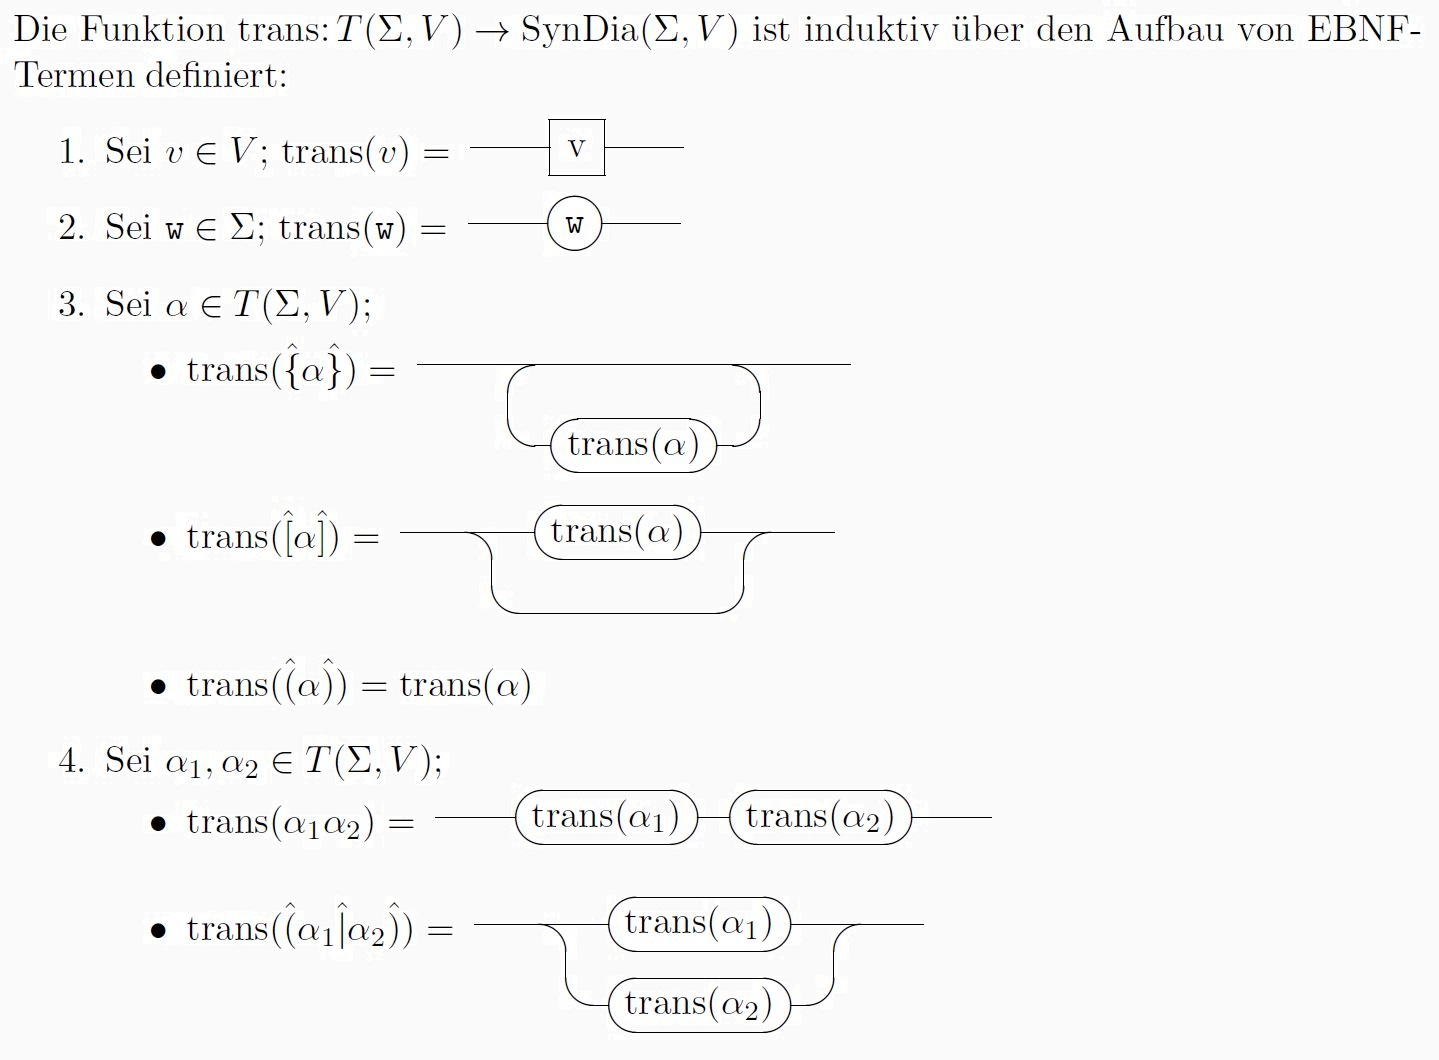
\includegraphics[width=.9\textwidth]{tut03_trans.jpg}
\end{frame}

\begin{frame} \frametitle{Semantik von EBNF-Termen}
	\begin{itemize}
		\item Sei $\mathcal{E} = (V,\Sigma,S,R)$ eine EBNF-Definition.
		\item $v \in V \leadsto W(\mathcal{E},v) = \rho(v)$ (syntaktische Kategorie)
		\item Semantik $\abb{\sem{\cdot}}{\underbrace{T(\Sigma, V)}_{\alpha}}{((\underbrace{V \to \pows{\Sigma^\ast}}_{\rho}) \to \pows{\Sigma^\ast})}$
		\item[] 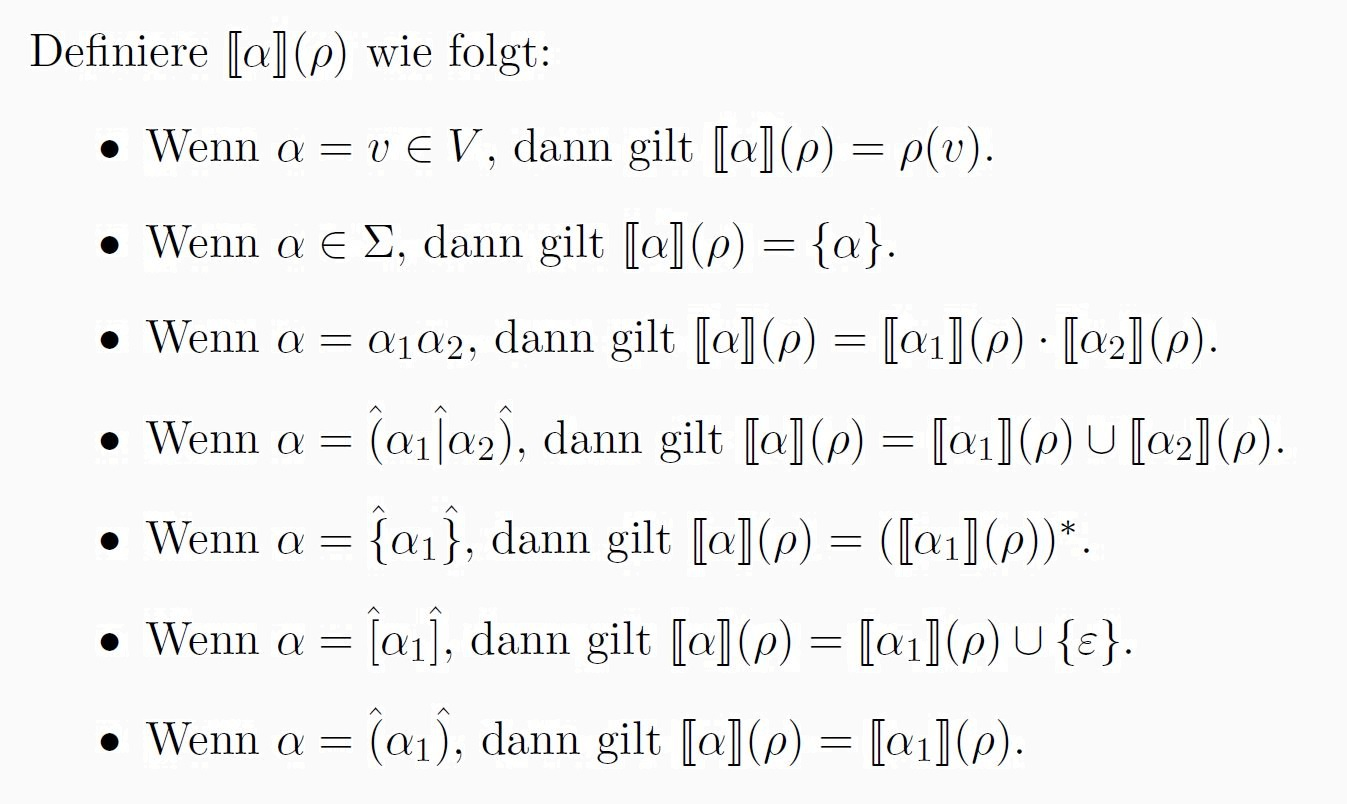
\includegraphics[width=.9\textwidth]{tut03_semantik.jpg}
	\end{itemize}	
\end{frame}

\section{Übungsblatt 3}

\begin{frame} \frametitle{Aufgabe 1 --- Teil (a)}
	\textbf{Gegeben} sei eine EBNF-Definition $\mathcal{E} = (V,\Sigma, S, R)$ mit $V= \menge{S,A,B}$, $\Sigma = \menge{a,b,c,d}$ und 
	\begin{equation*}
		R = \menge{ \quad S ::= AB, \quad A ::= \opt{aAc}{\wdh{b}}, \quad B ::= d \byp{B} c \quad }
	\end{equation*}
	\textbf{Gesucht} ist ein System von Syntaxdiagrammen
	
	\pause \centering
	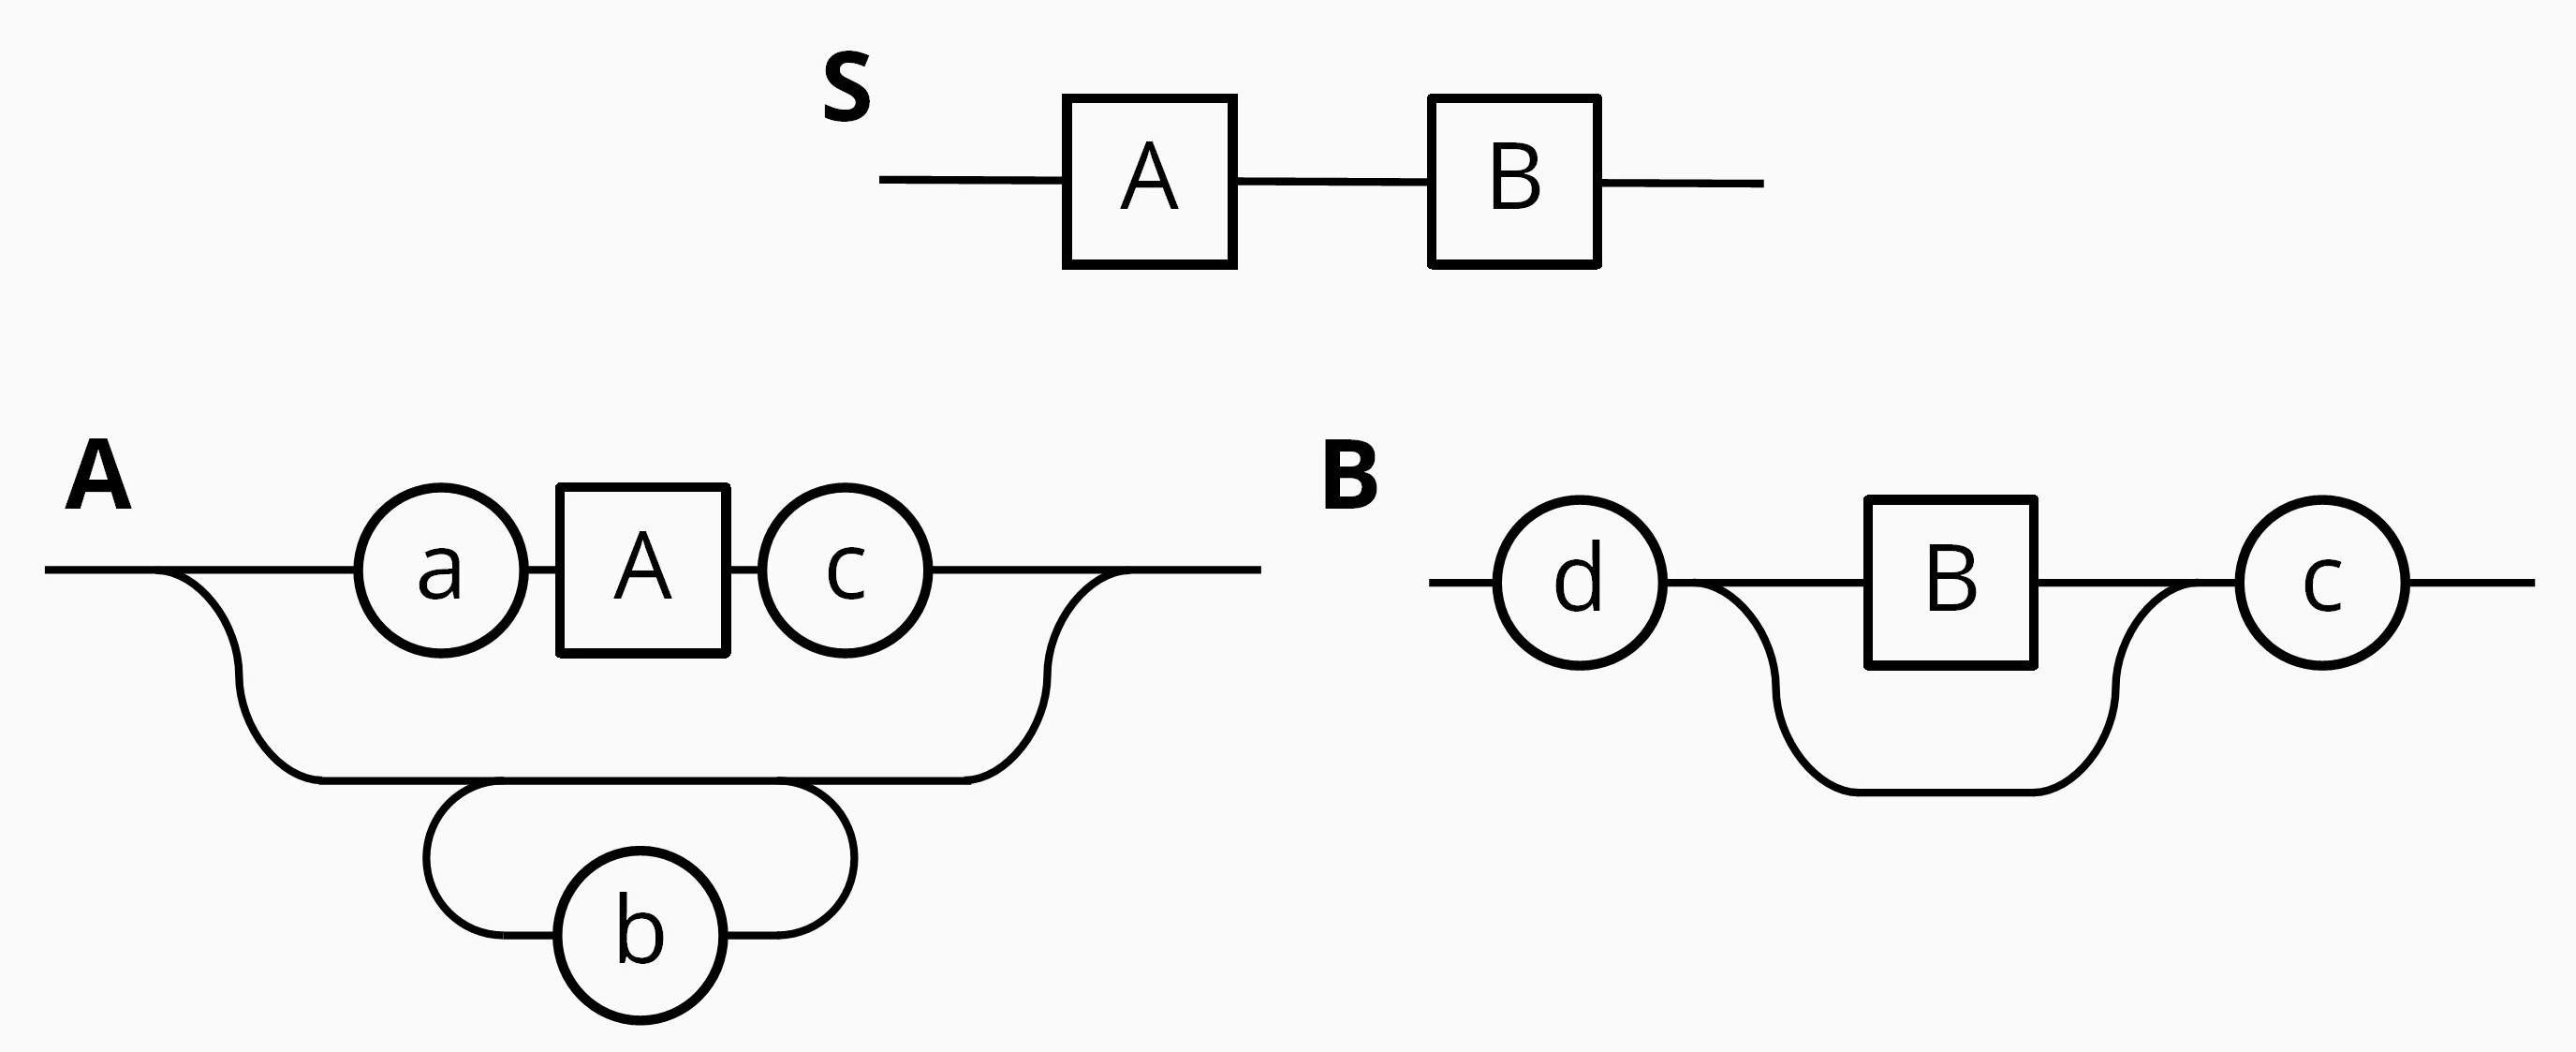
\includegraphics[width=\textwidth]{tut03_syntax_dia_1a.jpg}
\end{frame}

\begin{frame} \frametitle{Aufgabe 1 --- Teil (b)}
	\pause
	Wir wollen eine EBNF-Definition $\mathcal{E}' = (V,\Sigma,S,R)$ finden, sodass 
	\begin{align*}
		W(\mathcal{E}') &= \menge{a^{n+\ell} c b^n (cd)^\ell \mid n, \ell \in \N, n \ge 1}
		%
		\intertext{gilt. Wir zerlegen wie üblich die Sprache in unabhängige Teile:}
		%
		L &= \menge{\textcolor{cdpurple}{a^\ell} \enskip \textcolor{cdorange}{a^n} \ c \ \textcolor{cdorange}{b^n} \enskip \textcolor{cdpurple}{(cd)^\ell} \mid n,\ell \in \N, n \ge 1}
		%
		\intertext{Dann ergibt sich also nach dem Grundschema}
		%
		V &= \menge{S,A} \\
		R &= \menge{S ::= \opt{aScd}{A} , \enskip A ::= a \ \opt{A}{c} \ b}
	\end{align*}
\end{frame}

\begin{frame} \frametitle{Semantik von EBNF-Termen}
	\begin{itemize}
		\item Sei $\mathcal{E} = (V,\Sigma,S,R)$ eine EBNF-Definition.
		\item $v \in V \leadsto W(\mathcal{E},v) = \rho(v)$ (syntaktische Kategorie)
		\item Semantik $\abb{\sem{\cdot}}{\underbrace{T(\Sigma, V)}_{\alpha}}{((\underbrace{V \to \pows{\Sigma^\ast}}_{\rho}) \to \pows{\Sigma^\ast})}$
		\item[] 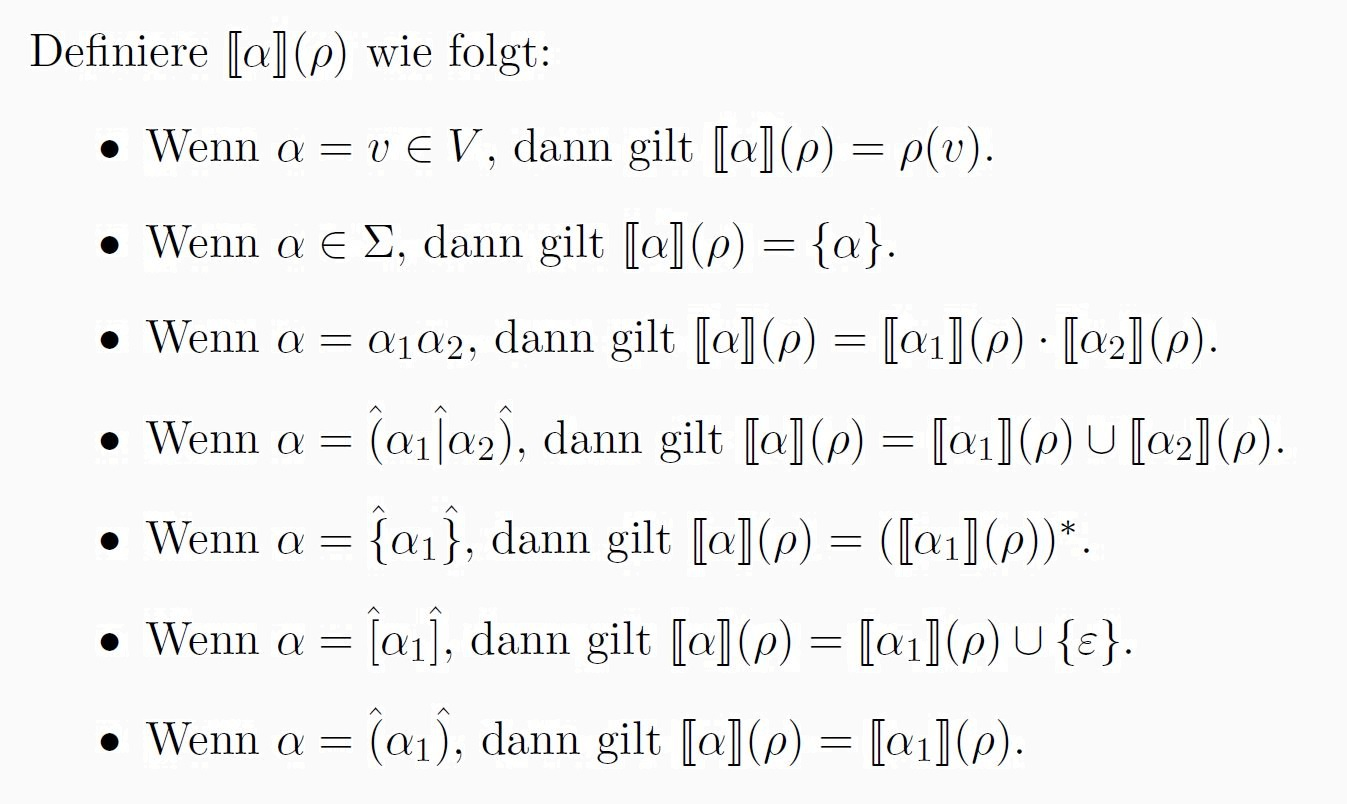
\includegraphics[width=.9\textwidth]{tut03_semantik.jpg}
	\end{itemize}	
\end{frame}

\begin{frame} \frametitle{Aufgabe 2 --- Teil (a)}
	\begin{itemize}
		\item $\rho \colon V \to \pows{\Sigma^\ast}$
		\item $f \colon (V \to \pows{\Sigma^\ast}) \to (V \to \pows{\Sigma^\ast})$
	\end{itemize}
	\pause
	\begin{align*}
		f(\rho) = \begin{pmatrix} f(\rho)(S) \\ f(\rho)(A) \end{pmatrix} 
		= \begin{pmatrix} \sem{ddAc}(\rho) \\ \sem{\byp{S}a}(\rho) \end{pmatrix} 
		&= \begin{pmatrix}
			\menge{dd} * \rho(A) * \menge{c} \\ \brackets{\rho(S) \cup \menge{\epsilon}} * \menge{a}
		\end{pmatrix} \\
		&= \begin{pmatrix}
			\menge{dd} * \rho(A) * \menge{c} \\ \rho(S) * \menge{a} \cup \menge{a}
		\end{pmatrix}
	\end{align*}
\end{frame}

\begin{frame} \frametitle{Aufgabe 2 --- Teil (b)}
	\begin{equation*}
		f(\rho) = \begin{pmatrix}
			\menge{dd} * \rho(A) * \menge{c} \\ \rho(S) * \menge{a} \cup \menge{a}
		\end{pmatrix}
	\end{equation*}
	
	\begin{align*}
		\begin{pmatrix} \emptyset \\ \emptyset \end{pmatrix}
		\mapsto^1
		\begin{pmatrix} \emptyset \\ \menge{a} \end{pmatrix}
		\mapsto^2
		\begin{pmatrix} \menge{ddac} \\ \menge{a} \end{pmatrix}
		&\mapsto^3
		\begin{pmatrix} \menge{ddac} \\ \menge{ddaca,a} \end{pmatrix} \\
		&\mapsto^4
		\begin{pmatrix} \menge{(dd)^2 (ac)^2, ddac} \\ \menge{ddaca, a} \end{pmatrix} \\
		&\mapsto^5
		\begin{pmatrix} \menge{(dd)^2 (ac)^2, ddac} \\ \menge{(dd)^2 (ac)^2 a, ddaca, a} \end{pmatrix}
	\end{align*}
\end{frame}

\begin{frame} \frametitle{Aufgabe 2 --- Teil (c)}
	Die ersten Schritte zeigten 
	\begin{equation*}
		\begin{pmatrix} \emptyset \\ \emptyset \end{pmatrix}
		\mapsto^1 \cdots \mapsto^5
		\begin{pmatrix} \menge{(dd)^2 (ac)^2, ddac} \\ \menge{(dd)^2 (ac)^2 a, ddaca, a} \end{pmatrix}
	\end{equation*}
	
	Führen wir diese Iteration nur \enquote{bis ins Unendliche} fort, so erhalten wir
	\begin{align*}
		W(\mathcal{E}, S) &= \menge{(dd)^n (ac)^n : n \ge 1} \\
		W(\mathcal{E}, A) &= \menge{(dd)^n (ac)^n a : n \ge 0}
	\end{align*}
\end{frame}


\begin{frame} \frametitle{Aufgabe 3 --- Teil (a)}
	Wir brauchen die Semantik von $S ::= \byp{a\opt{Sb}{Sbb}}$.
	\pause
		\begin{align*}
		\sem{\byp{a \opt{Sb}{Sbb}}}(\rho)
		&= \menge{\epsilon} \cup \sem{a \opt{Sb}{Sbb}}(\rho) \\
		&= \menge{\epsilon} \cup \menge{a} * \sem{\opt{Sb}{Sbb}}(\rho) \\
		&= \menge{\epsilon} \cup \menge{a} * \brackets{\sem{Sb}(\rho) \cup \sem{Sbb}(\rho)} \\
		&= \menge{\epsilon} \cup \menge{a} * \brackets{\rho(S) * \menge{b} \cup \rho(S) * \menge{bb}} \\
		&= \menge{\epsilon} \cup \menge{a} * \rho(S) * \menge{b} \cup \menge{a} * \rho(S) * \menge{bb}
	\end{align*}
	\pause
	Damit können wir die Iterationsfunktion aufstellen:
	\begin{align*}
		f(\rho) = \begin{pmatrix} f(\rho)(S) \end{pmatrix} 
		&= \begin{pmatrix} \sem{\byp{a \opt{Sb}{Sbb}}}(\rho) \end{pmatrix} \\
		&= \begin{pmatrix}
			\menge{\epsilon} \cup \menge{a} * \rho(S) * \menge{b} \cup \menge{a} * \rho(S) * \menge{bb}
		\end{pmatrix}
	\end{align*}
\end{frame}

\begin{frame} \frametitle{Aufgabe 3 --- Teil (a)}
	\begin{equation*}
		f(\rho) = \begin{pmatrix}
			\menge{\epsilon} \cup \menge{a} * \rho(S) * \menge{b} \cup \menge{a} * \rho(S) * \menge{bb}
		\end{pmatrix}
	\end{equation*}
	\pause
	
	\textbf{3 Iterationen:}
	\begin{align*}
		\begin{pmatrix} \emptyset \end{pmatrix}
		\mapsto^1
		\begin{pmatrix} \menge{\epsilon} \end{pmatrix}
		&\mapsto^2
		\begin{pmatrix} \menge{\epsilon, ab, abb} \end{pmatrix} \\
		&\mapsto^3
		\begin{pmatrix} \menge{\epsilon, ab, abb, aabb, aabbb, aabbbb} \end{pmatrix}
	\end{align*}
\end{frame}



\begin{frame} \frametitle{Aufgabe 3 --- Teil (b)}
	\small 
	Sei $\rho \colon V \to \pows{\Sigma^\ast}$ mit $\rho(S) = \menge{a^n b^n \mid 2n \ge m \ge n \ge 0}$. 
		
	\textbf{Zu zeigen:} $\sem{\byp{a \opt{Sb}{Sbb}}}(\rho) = \rho(S)$.
	
	\pause
	
	\begin{align*}
		&\sem{\byp{a \opt{Sb}{Sbb}}}(\rho) \\
		= \enskip & \menge{\epsilon} \cup \menge{a} * \rho(S) * \menge{b} \cup \menge{a} * \rho(S) * \menge{bb} \\
		= \enskip & \scalebox{0.8}{ $\menge{\epsilon} \cup \menge{a} * \menge{a^n b^n \mid 2n \ge m \ge n \ge 0} * \menge{b} \cup \menge{a} * \menge{a^n b^n \mid 2n \ge m \ge n \ge 0} * \menge{bb} $} \\
		= \enskip & \menge{\epsilon} \cup \menge{a a^n b^n b \mid 2n \ge m \ge n \ge 0} \cup \menge{a a^n b^m bb \mid 2n \ge m \ge n \ge 0}  \\
		= \enskip & \menge{a^n b^m \mid 2n \ge m \ge n \ge 0} \\
		= \enskip & \rho(S)
	\end{align*}
\end{frame}



\end{document}